%%%%%%%%%%%%%%%%%%%%%%%%%%%%%%%%%%%%%%%%%%%%%%%%%%%%%%%%%%%%%%%%%%%%%%%%%%%%%%%
%%%    Overview for Chen/Stetina/Wildman Capstone project
%%%%%%%%%%%%%%%%%%%%%%%%%%%%%%%%%%%%%%%%%%%%%%%%%%%%%%%%%%%%%%%%%%%%%%%%%%%%%%%

%------------------------------------------------------------------------------
%	PACKAGES AND DOCUMENT OPTIONS
%------------------------------------------------------------------------------

%Page options
\documentclass[paper=a4, fontsize=12pt]{article}
\usepackage[margin=1in]{geometry}

%Font options
%\usepackage{fontspec}

%Math packages
\usepackage{amsmath}
\usepackage{amsfonts}
\usepackage{amsthm}
\usepackage{bm}

%Graphics packages
\usepackage{graphicx}
\usepackage{subcaption}
\usepackage{tikz}
\usetikzlibrary{shapes,arrows,chains,calc}

%Section options
\usepackage{sectsty}
\allsectionsfont{\normalfont \scshape}

%Bibliography options
% \usepackage[backend=biber,style=chem-acs]{biblatex}

%Custom commands
\renewcommand{\abstractname}{\Large Summary}
\newcommand{\softname}{\texttt{graph\_energy}}

%------------------------------------------------------------------------------
%	TITLE
%------------------------------------------------------------------------------

\title{
\softname\ Overview
}

\author{You Chen, Torin Stetina, Andrew Wildman}

\date{May 3, 2018}

\begin{document}

\maketitle

%------------------------------------------------------------------------------
%	BODY
%------------------------------------------------------------------------------

\begin{abstract}
  The goal of this project is twofold:
  \begin{enumerate}
    \item Develop a software framework that predicts the energy distribution of a group of microstates from their topological parameters
    \item Validate this framework on two sets of example data,
      specifically an ideal ice model and a lattice gas model.
  \end{enumerate}
\end{abstract}

\section*{Motivation}

% TODO: Motivation

\section*{Approach}

% TODO: Motivate graph energy

The central prediction capabilities of \softname\ are provided through a machine learning algorithm.
Because the relationship between the graph connections and the energy is expected to be non-linear,
(e.g. for a hydrogen bond graph, four edges on a node will likely be lower in energy than three or five)
a simple, feed forward neural net has been chosen as the prediction algorithm.
Neural networks have a large meta-parameter space,
so an optimization of these meta-parameters will be built into the software itself.

\subsection*{Use Cases}

The \softname\ package has four main use cases:

\begin{enumerate}
  \item Train a neural net to reproduce the energy distribution of a set of microstates,
    given graph topological parameters that define the microstate, temperature, and population of the microstate at that temperature.
  \item Evaluate the accuracy of nets trained on different sets of topological parameters at capturing the energy distribution. 
  \item Use previously trained neural nets to predict the energy distribution of microstates whose energy distribution was previously unknown.
  \item Visualize the predicted energy distribution and, if available, contrast it with the known energy distribution.
\end{enumerate}

\subsection*{Data Description}

\textbf{Note:} This section is out of date once we get the new output that includes the true microstate energy.

% TODO: Update data description

\vspace{1em}

\noindent The raw data comes from the Clark Group's Shannon entropy program.
It consists of a set of \texttt{output.dat}\ files,
each of which is generated at a given temperature
and contain the topological parameter values of each microstate, as well as the population at that temperature.
An example of an \text{output.dat} file is given in figure \ref{output}.

\begin{figure}
  \centering
  \includegraphics[width=0.8\textwidth]{output_file}
  \caption[width=0.8\textwidth]{An example output file from the Clark Group's Shannon entropy program}
  \label{output}
\end{figure}

% TODO: Input file spec

\section*{Software Design}

\newpage

\subsection*{Software flow}

% Main module software flow. Based on: 
%     Flowcharting techniques for easy maintenance
%     Original Author: Brent Longborough
%     Retreived from : http://www.texample.net/tikz/examples/flexible-flow-chart/
%     Retreived on: April 26, 2018
% =================================================
% -------------------------------------------------
% Set up a new layer for the debugging marks, and make sure it is on
% top
\pgfdeclarelayer{marx}
\pgfsetlayers{main,marx}
% A macro for marking coordinates (specific to the coordinate naming
% scheme used here). Swap the following 2 definitions to deactivate
% marks.
\providecommand{\cmark}[2][]{%
  \begin{pgfonlayer}{marx}
    \node [nmark] at (c#2#1) {#2};
  \end{pgfonlayer}{marx}
  } 
\providecommand{\cmark}[2][]{\relax} 

% =================================================
% -------------------------------------------------
% Start the picture
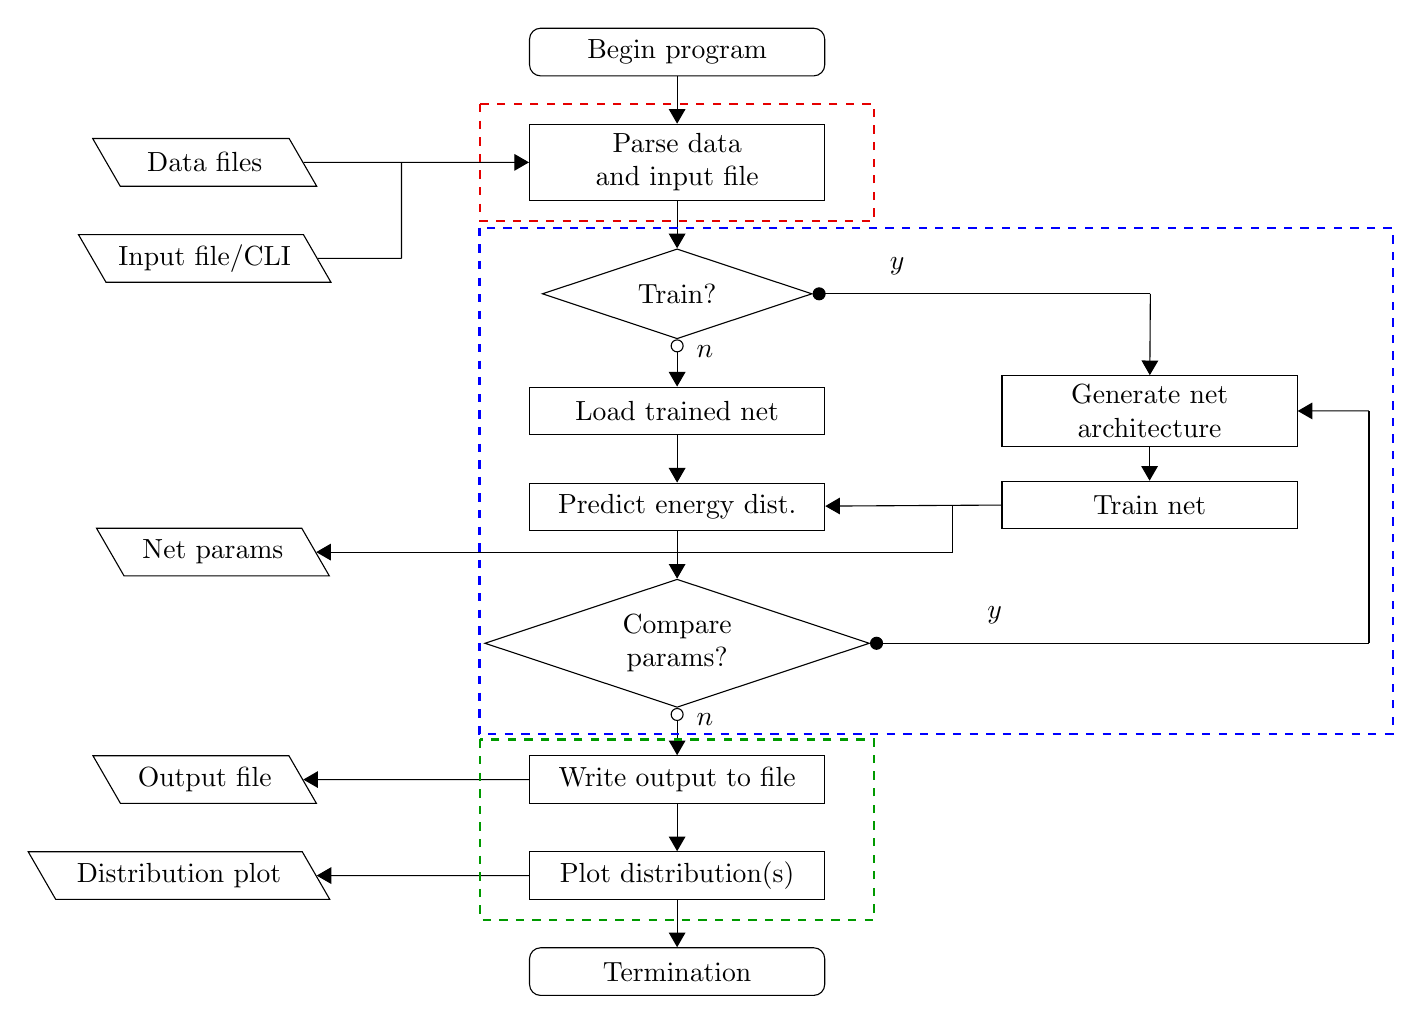
\begin{tikzpicture}[%
    >=triangle 60,              % Nice arrows; your taste may be different
    start chain=going below,    % General flow is top-to-bottom
    node distance=6mm and 60mm, % Global setup of box spacing
    every join/.style={norm},   % Default linetype for connecting boxes
    ]
% ------------------------------------------------- 
% A few box styles 
% <on chain> *and* <on grid> reduce the need for manual relative
% positioning of nodes
\tikzset{
  base/.style={draw, on chain, on grid, align=center, minimum height=4ex},
  proc/.style={base, rectangle, text width=10em},
  test/.style={base, diamond, aspect=3, text width=5em},
  term/.style={proc, rounded corners},
  inpt/.style={base, trapezium, trapezium left angle=120, trapezium right angle=60},
  % coord node style is used for placing corners of connecting lines
  coord/.style={coordinate, on chain, on grid, node distance=6mm and 25mm},
  % nmark node style is used for coordinate debugging marks
  nmark/.style={draw, cyan, circle, font={\sffamily\bfseries}},
  % -------------------------------------------------
  % Connector line styles for different parts of the diagram
  norm/.style={->}
}
% -------------------------------------------------
% Place the nodes
\node [term] (start) {Begin program};
\node [proc, join] (p1) {Parse data and input file};
\node [test, join] (t1) {Train?};
\node [proc] (p2) {Load trained net};
\node [proc, join] (p3) {Predict energy dist.};
\node [test, join] (t2) {Compare params?};
\node [proc] (p4) {Write output to file};
\node [proc, join] (p4d) {Plot distribution(s)};
\node [term, join] {Termination};

% Side nodes
\node [inpt, left=of p1] (i1) {Data files};
\node [inpt] (i2) {Input file/CLI}; 

\node[inpt, left=of p4] (i3) {Output file};
\node[inpt, left=18em of p4d] (i4) {Distribution plot};

\node [proc, right=of p2] (p5) {Generate net architecture};
\node [proc, below=3.4em of p5, join] (p6) {Train net};

% Invisible corner nodes
\node [coord, right=of i1] (c1) {}; % \cmark{1};
\node [coord, right=of i2] (c2) {}; % \cmark{2};
\node [coord, right=17.1em of t1] (c3) {}; % \cmark{3};
\node [coord, right=25em of t2] (c4) {}; % \cmark{4};
\node [coord, above=8.4em of c4] (c5) {}; % \cmark{5};
\node [coord, left=of p6] (c6) {}; % \cmark{6};
\node [coord, below=1.7em of c6] (c7) {}; % \cmark{7};

% One last output node
\node [inpt, left=23em of c7] (i5) {Net params};

% Simple left/right connections
\draw [->] (i1.east) -- (p1);
\draw [->] (p6.west) -- (p3);
\draw [->] (p4.west) -- (i3);
\draw [->] (p4d.west) -- (i4);

% Simple top/bottom connections
\path (t1.south) to node [near start, xshift=1em] {$n$} (p2);
\draw [o->] (t1.south) -- (p2);

\path (t2.south) to node [near start, xshift=1em] {$n$} (p4);
\draw [o->] (t2.south) -- (p4);

% Corner paths
\draw[-] (i2.east) -- (c2);
\draw[-] (c2) -- (c1);

\path (t1.east) to node [near start, yshift=1em] {$y$} (c3);
\draw[*-] (t1.east) -- (c3);
\draw[->] (c3) -- (p5);

\path (t2.east) to node [near start, yshift=1em] {$y$} (c4);
\draw[*-] (t2.east) -- (c4);
\draw[-] (c4) -- (c5);
\draw[->] (c5) -- (p5.east);

\draw[-] (c6) -- (c7);
\draw[->] (c7) -- (i5.east);

% Boxes
\draw[black!10!red,thick,dashed] ($(p1.north west)+(-0.62,0.25)$) rectangle ($(p1.south east)+(0.62,-0.25)$); 
\draw[blue,thick,dashed] ($(t1.north west)+(-1.65,0.55)$) rectangle ($(c4)+(0.3,-1.15)$);
\draw[black!40!green,thick,dashed] ($(p4.north west)+(-0.62,0.2)$) rectangle ($(p4d.south east)+(0.62,-0.25)$);

\end{tikzpicture}


The rhombuses represent inputs or outputs to the program,
rectangles represent processes,
diamonds represent tests,
and rounded boxes delimit the bounds of the program.
The dashed boxes represent software components/classes, which will be described in the next section.

\subsection*{Component specification}

{\noindent \large \textbf{Parser} }

The parser takes the \texttt{output.dat} files as well as the input file,
then it converts them into the expected inputs for the parser. 
 
\underline{Input file}:
\begin{itemize}
  \item \texttt{/path/to/output.dat}
  \item Job type: \texttt{train} or \texttt{predict}
  \item Meta parameter options for neural net
\end{itemize}

\underline{Outputs}:
\begin{itemize}
  \item Dataframe object from columns of \texttt{output.dat}
  \item Dictionary of meta parameters and job type for neural net
\end{itemize}

\underline{Exceptions}:
\begin{itemize}
  \item Handle wrong \texttt{.dat} file format
  \item Handle input file format errors
\end{itemize}


{\noindent \large \textbf{Predictor} }

% TODO: Predictor spec

%\begin{itemize}
%  \underline{Possible Inputs}:
%  \item 
%
%  \underline{Outputs}:
%  \item 
%
%  \underline{Exceptions}:
%  \item
%\end{itemize}

{\noindent \large \textbf{Visualizer} }

% TODO: Visualizer spec

%\begin{itemize}
%  \underline{Possible Inputs}:
%  \item 
%
%  \underline{Outputs}:
%  \item 
%
%  \underline{Exceptions}:
%  \item
%\end{itemize}

\end{document}
